% Created by tikzDevice version 0.12.3.1 on 2022-11-29 09:22:03
% !TEX encoding = UTF-8 Unicode
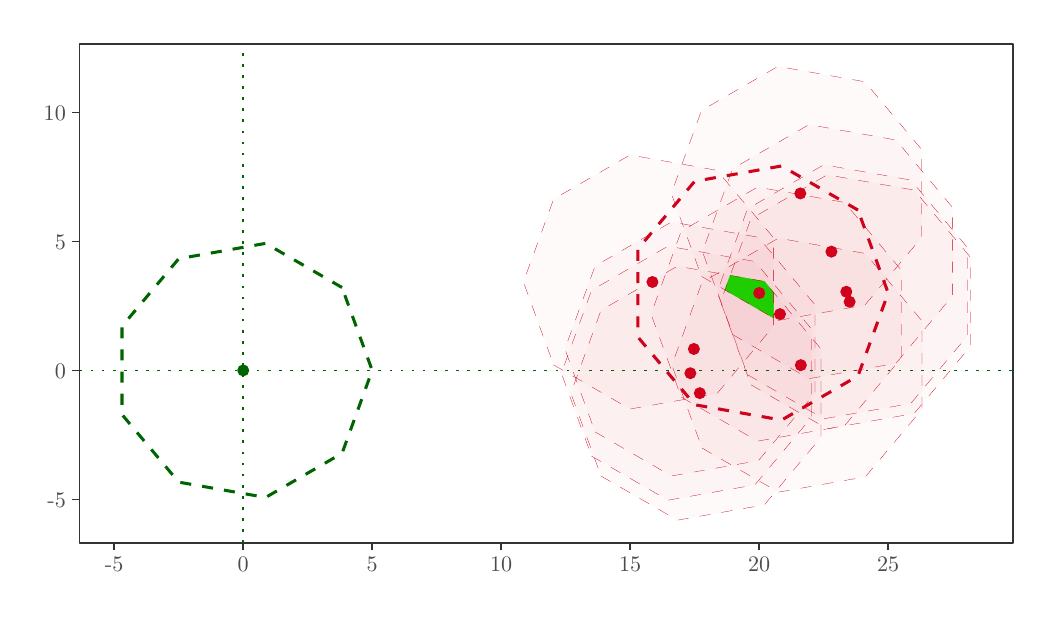
\begin{tikzpicture}[x=1pt,y=1pt]
\definecolor{fillColor}{RGB}{255,255,255}
\begin{scope}
\definecolor{drawColor}{RGB}{255,255,255}
\definecolor{fillColor}{RGB}{255,255,255}

\path[draw=drawColor,line width= 0.6pt,line join=round,line cap=round,fill=fillColor] (  0.00, 78.98) rectangle (361.35,282.37);
\end{scope}
\begin{scope}
\definecolor{fillColor}{RGB}{255,255,255}

\path[fill=fillColor] ( 18.45, 96.50) rectangle (355.85,276.87);
\definecolor{drawColor}{RGB}{0,100,0}

\path[draw=drawColor,line width= 1.1pt,dash pattern=on 4pt off 4pt ,line join=round,even odd rule]
	(113.29,188.78) --
	( 85.68,204.72) --
	( 54.28,199.18) --
	( 33.78,174.76) --
	( 33.78,142.88) --
	( 54.28,118.45) --
	( 85.68,112.92) --
	(113.29,128.86) --
	(124.19,158.82) --
	(113.29,188.78) --
	cycle;
\definecolor{fillColor}{RGB}{0,100,0}

\path[draw=drawColor,line width= 0.4pt,line join=round,fill=fillColor] ( 77.58,158.82) circle (  1.96);
\definecolor{drawColor}{RGB}{208,2,28}

\path[draw=drawColor,line width= 1.1pt,dash pattern=on 4pt off 4pt ,line join=round,even odd rule]
	(299.73,216.75) --
	(272.12,232.69) --
	(240.72,227.15) --
	(220.23,202.73) --
	(220.23,170.84) --
	(240.72,146.42) --
	(272.12,140.88) --
	(299.73,156.82) --
	(310.64,186.78) --
	(299.73,216.75) --
	cycle;
\definecolor{drawColor}{RGB}{0,255,0}
\definecolor{fillColor}{RGB}{0,255,0}

\path[draw=drawColor,line width= 0.2pt,line join=round,fill=fillColor,even odd rule]
	(265.89,190.97) --
	(269.25,186.96) --
	(269.25,177.76) --
	(251.67,187.91) --
	(253.57,193.14) --
	(265.89,190.97) --
	cycle;
\definecolor{drawColor}{RGB}{0,100,0}

\path[draw=drawColor,line width= 0.6pt,dash pattern=on 1pt off 3pt ,line join=round] ( 18.45,158.82) -- (355.85,158.82);

\path[draw=drawColor,line width= 0.6pt,dash pattern=on 1pt off 3pt ,line join=round] ( 77.58, 96.50) -- ( 77.58,276.87);
\definecolor{drawColor}{RGB}{208,2,28}
\definecolor{fillColor}{RGB}{208,2,28}

\path[draw=drawColor,line width= 0.4pt,line join=round,fill=fillColor] (264.03,186.78) circle (  1.96);

\path[draw=drawColor,line width= 0.4pt,line join=round,fill=fillColor] (296.71,183.61) circle (  1.96);

\path[draw=drawColor,line width= 0.4pt,line join=round,fill=fillColor] (242.58,150.60) circle (  1.96);

\path[draw=drawColor,line width= 0.4pt,line join=round,fill=fillColor] (240.43,166.57) circle (  1.96);

\path[draw=drawColor,line width= 0.4pt,line join=round,fill=fillColor] (225.45,190.77) circle (  1.96);

\path[draw=drawColor,line width= 0.4pt,line join=round,fill=fillColor] (279.08,160.72) circle (  1.96);

\path[draw=drawColor,line width= 0.4pt,line join=round,fill=fillColor] (278.89,222.77) circle (  1.96);

\path[draw=drawColor,line width= 0.4pt,line join=round,fill=fillColor] (239.16,157.81) circle (  1.96);

\path[draw=drawColor,line width= 0.4pt,line join=round,fill=fillColor] (271.55,179.16) circle (  1.96);

\path[draw=drawColor,line width= 0.4pt,line join=round,fill=fillColor] (295.51,187.24) circle (  1.96);

\path[draw=drawColor,line width= 0.4pt,line join=round,fill=fillColor] (290.13,201.74) circle (  1.96);
\definecolor{fillColor}{RGB}{208,2,28}

\path[draw=drawColor,line width= 0.1pt,dash pattern=on 4pt off 4pt ,line join=round,fill=fillColor,fill opacity=0.02,even odd rule]
	(261.01,153.65) --
	(288.62,137.71) --
	(320.02,143.24) --
	(340.51,167.67) --
	(340.51,199.55) --
	(320.02,223.98) --
	(288.62,229.51) --
	(261.01,213.57) --
	(250.10,183.61) --
	(261.01,153.65) --
	cycle;

\path[draw=drawColor,line width= 0.1pt,dash pattern=on 4pt off 4pt ,line join=round,fill=fillColor,fill opacity=0.02,even odd rule]
	(206.88,120.64) --
	(234.49,104.70) --
	(265.89,110.23) --
	(286.38,134.66) --
	(286.38,166.54) --
	(265.89,190.97) --
	(234.49,196.50) --
	(206.88,180.56) --
	(195.97,150.60) --
	(206.88,120.64) --
	cycle;

\path[draw=drawColor,line width= 0.1pt,dash pattern=on 4pt off 4pt ,line join=round,fill=fillColor,fill opacity=0.02,even odd rule]
	(204.72,136.61) --
	(232.34,120.67) --
	(263.74,126.20) --
	(284.23,150.63) --
	(284.23,182.51) --
	(263.74,206.93) --
	(232.34,212.47) --
	(204.72,196.53) --
	(193.82,166.57) --
	(204.72,136.61) --
	cycle;

\path[draw=drawColor,line width= 0.1pt,dash pattern=on 4pt off 4pt ,line join=round,fill=fillColor,fill opacity=0.02,even odd rule]
	(189.75,160.81) --
	(217.36,144.86) --
	(248.76,150.40) --
	(269.25,174.82) --
	(269.25,206.71) --
	(248.76,231.13) --
	(217.36,236.67) --
	(189.75,220.73) --
	(178.84,190.77) --
	(189.75,160.81) --
	cycle;

\path[draw=drawColor,line width= 0.1pt,dash pattern=on 4pt off 4pt ,line join=round,fill=fillColor,fill opacity=0.02,even odd rule]
	(243.37,130.76) --
	(270.98,114.82) --
	(302.38,120.35) --
	(322.88,144.78) --
	(322.88,176.66) --
	(302.38,201.08) --
	(270.98,206.62) --
	(243.37,190.68) --
	(232.47,160.72) --
	(243.37,130.76) --
	cycle;

\path[draw=drawColor,line width= 0.1pt,dash pattern=on 4pt off 4pt ,line join=round,fill=fillColor,fill opacity=0.02,even odd rule]
	(243.18,192.80) --
	(270.80,176.86) --
	(302.20,182.40) --
	(322.69,206.82) --
	(322.69,238.71) --
	(302.20,263.13) --
	(270.80,268.67) --
	(243.18,252.73) --
	(232.28,222.77) --
	(243.18,192.80) --
	cycle;

\path[draw=drawColor,line width= 0.1pt,dash pattern=on 4pt off 4pt ,line join=round,fill=fillColor,fill opacity=0.02,even odd rule]
	(203.46,127.85) --
	(231.07,111.91) --
	(262.47,117.45) --
	(282.96,141.87) --
	(282.96,173.76) --
	(262.47,198.18) --
	(231.07,203.72) --
	(203.46,187.77) --
	(192.55,157.81) --
	(203.46,127.85) --
	cycle;

\path[draw=drawColor,line width= 0.1pt,dash pattern=on 4pt off 4pt ,line join=round,fill=fillColor,fill opacity=0.02,even odd rule]
	(235.85,149.20) --
	(263.46,133.26) --
	(294.86,138.79) --
	(315.35,163.22) --
	(315.35,195.10) --
	(294.86,219.53) --
	(263.46,225.06) --
	(235.85,209.12) --
	(224.94,179.16) --
	(235.85,149.20) --
	cycle;

\path[draw=drawColor,line width= 0.1pt,dash pattern=on 4pt off 4pt ,line join=round,fill=fillColor,fill opacity=0.02,even odd rule]
	(259.80,157.28) --
	(287.41,141.34) --
	(318.81,146.87) --
	(339.31,171.30) --
	(339.31,203.18) --
	(318.81,227.61) --
	(287.41,233.14) --
	(259.80,217.20) --
	(248.90,187.24) --
	(259.80,157.28) --
	cycle;

\path[draw=drawColor,line width= 0.1pt,dash pattern=on 4pt off 4pt ,line join=round,fill=fillColor,fill opacity=0.02,even odd rule]
	(254.43,171.78) --
	(282.04,155.83) --
	(313.44,161.37) --
	(333.93,185.79) --
	(333.93,217.68) --
	(313.44,242.10) --
	(282.04,247.64) --
	(254.43,231.70) --
	(243.52,201.74) --
	(254.43,171.78) --
	cycle;
\definecolor{drawColor}{gray}{0.20}

\path[draw=drawColor,line width= 0.6pt,line join=round,line cap=round] ( 18.45, 96.50) rectangle (355.85,276.87);
\end{scope}
\begin{scope}
\definecolor{drawColor}{gray}{0.30}

\node[text=drawColor,anchor=base east,inner sep=0pt, outer sep=0pt, scale=  0.80] at ( 13.50,109.45) { -5};

\node[text=drawColor,anchor=base east,inner sep=0pt, outer sep=0pt, scale=  0.80] at ( 13.50,156.06) {  0};

\node[text=drawColor,anchor=base east,inner sep=0pt, outer sep=0pt, scale=  0.80] at ( 13.50,202.67) {  5};

\node[text=drawColor,anchor=base east,inner sep=0pt, outer sep=0pt, scale=  0.80] at ( 13.50,249.28) { 10};
\end{scope}
\begin{scope}
\definecolor{drawColor}{gray}{0.20}

\path[draw=drawColor,line width= 0.6pt,line join=round] ( 15.70,112.21) --
	( 18.45,112.21);

\path[draw=drawColor,line width= 0.6pt,line join=round] ( 15.70,158.82) --
	( 18.45,158.82);

\path[draw=drawColor,line width= 0.6pt,line join=round] ( 15.70,205.43) --
	( 18.45,205.43);

\path[draw=drawColor,line width= 0.6pt,line join=round] ( 15.70,252.04) --
	( 18.45,252.04);
\end{scope}
\begin{scope}
\definecolor{drawColor}{gray}{0.20}

\path[draw=drawColor,line width= 0.6pt,line join=round] ( 30.97, 93.75) --
	( 30.97, 96.50);

\path[draw=drawColor,line width= 0.6pt,line join=round] ( 77.58, 93.75) --
	( 77.58, 96.50);

\path[draw=drawColor,line width= 0.6pt,line join=round] (124.19, 93.75) --
	(124.19, 96.50);

\path[draw=drawColor,line width= 0.6pt,line join=round] (170.81, 93.75) --
	(170.81, 96.50);

\path[draw=drawColor,line width= 0.6pt,line join=round] (217.42, 93.75) --
	(217.42, 96.50);

\path[draw=drawColor,line width= 0.6pt,line join=round] (264.03, 93.75) --
	(264.03, 96.50);

\path[draw=drawColor,line width= 0.6pt,line join=round] (310.64, 93.75) --
	(310.64, 96.50);
\end{scope}
\begin{scope}
\definecolor{drawColor}{gray}{0.30}

\node[text=drawColor,anchor=base,inner sep=0pt, outer sep=0pt, scale=  0.80] at ( 30.97, 86.04) { -5};

\node[text=drawColor,anchor=base,inner sep=0pt, outer sep=0pt, scale=  0.80] at ( 77.58, 86.04) {  0};

\node[text=drawColor,anchor=base,inner sep=0pt, outer sep=0pt, scale=  0.80] at (124.19, 86.04) {  5};

\node[text=drawColor,anchor=base,inner sep=0pt, outer sep=0pt, scale=  0.80] at (170.81, 86.04) { 10};

\node[text=drawColor,anchor=base,inner sep=0pt, outer sep=0pt, scale=  0.80] at (217.42, 86.04) { 15};

\node[text=drawColor,anchor=base,inner sep=0pt, outer sep=0pt, scale=  0.80] at (264.03, 86.04) { 20};

\node[text=drawColor,anchor=base,inner sep=0pt, outer sep=0pt, scale=  0.80] at (310.64, 86.04) { 25};
\end{scope}
\end{tikzpicture}
